\section{Results and Discussion}

\subsection{Comparing Aggregate Statistics of Community Structure}

We begin by examining the overall statistics for the communities inferred by OSLOM using the weightings defined in the previous sections. The number of communities by community type is given in Table~\ref{Table-comm_count}. We see that the topic- and interaction-based networks admit the most communities. The activity-based network admits the least number of communities.  One advantage of the OSLOM over many other community detection algorithms is that it explicitly accounts for singleton `communities': those nodes who do not belong to \emph{any} extant communities. This is especially important when a network is collected via a breadth-first search, as in our network, where we begin from a seed node and then branch out. Such a search, once terminated, will result in a collection of nodes on the periphery of the network that may not belong to any community in the core.

% See here
% 	http://arxiv.org/pdf/1202.2684v2.pdf
% for possible useful references on core-periphery networks.

The number of singletons by community type is also shown in Table~\ref{Table-comm_count}. We see that the topic- and interaction-based communities have the most singletons, with the activity-based community dominating this measure. This result for the activity-based community is an artifact of a property of the retweet/mention weighting: 717 of the users were removed in the process \textbf{TK: Fix after clarification from Elisa}.

\begin{table}[ht]
	\caption{Number of non-singleton communities and singletons by community type: S(tructural), A(ctivity -based), T(opic-based), and I(nteraction-based).}
	\centering
	\begin{tabular}{| c | c | c |}
		\hline Community Type & \# of Communities & \# of Singletons \\ \hline
		% Structural & 201 \\
		% Activity, Lag 1 & 101 \\
		% Activity, Lag 2 & 99 \\
		% Activity, Lag 3 & 106 \\
		% Activity, Lag 4 & 105 \\
		% Activity, Lag 5 & 107 \\
		% Activity, Lag 6 & 106 \\
		% Topic & 289 \\
		% Interaction & 252 \\ \hline
		S & 201 & 308 \\
		A, Lag 1 & 101 & 951 \\
		A, Lag 2 & 99 & 600 \\
		A, Lag 3 & 106 & 611 \\
		A, Lag 4 & 105 & 668 \\
		A, Lag 5 & 107 & 632 \\
		A, Lag 6 & 106 & 642 \\
		T & 289 & 1064 \\
		I & 252 & 2436 (1719) \\ \hline
	\end{tabular}
	\label{Table-comm_count}
\end{table}

Next we consider the distribution of community sizes across the community types. The complementary cumulative distribution of community sizes is given in Figure~\ref{Fig-community_size_distribution}. Note that both axes are plotted on log-scale, and the horizontal axis begins with non-singleton communities. Thus, for a fixed community size $c$, Figure~\ref{Fig-community_size_distribution} shows the proportion of communities of size greater than $c$ for each community type. We see that the community distributions have longer tails for the non-structural networks, and that the interaction-based network has the longest tail. The largest communities for the structural, activity-based, topic-based, and interaction-based networks have 198, 358, 338, and 811 members, respectively. Most importantly, we see that the distributions are heterogeneous across the network types, highlighting that the different networks give rise to different large-scale community structure dependent on the particular weighting of the structural network.

\begin{figure}[ht]
  \centering
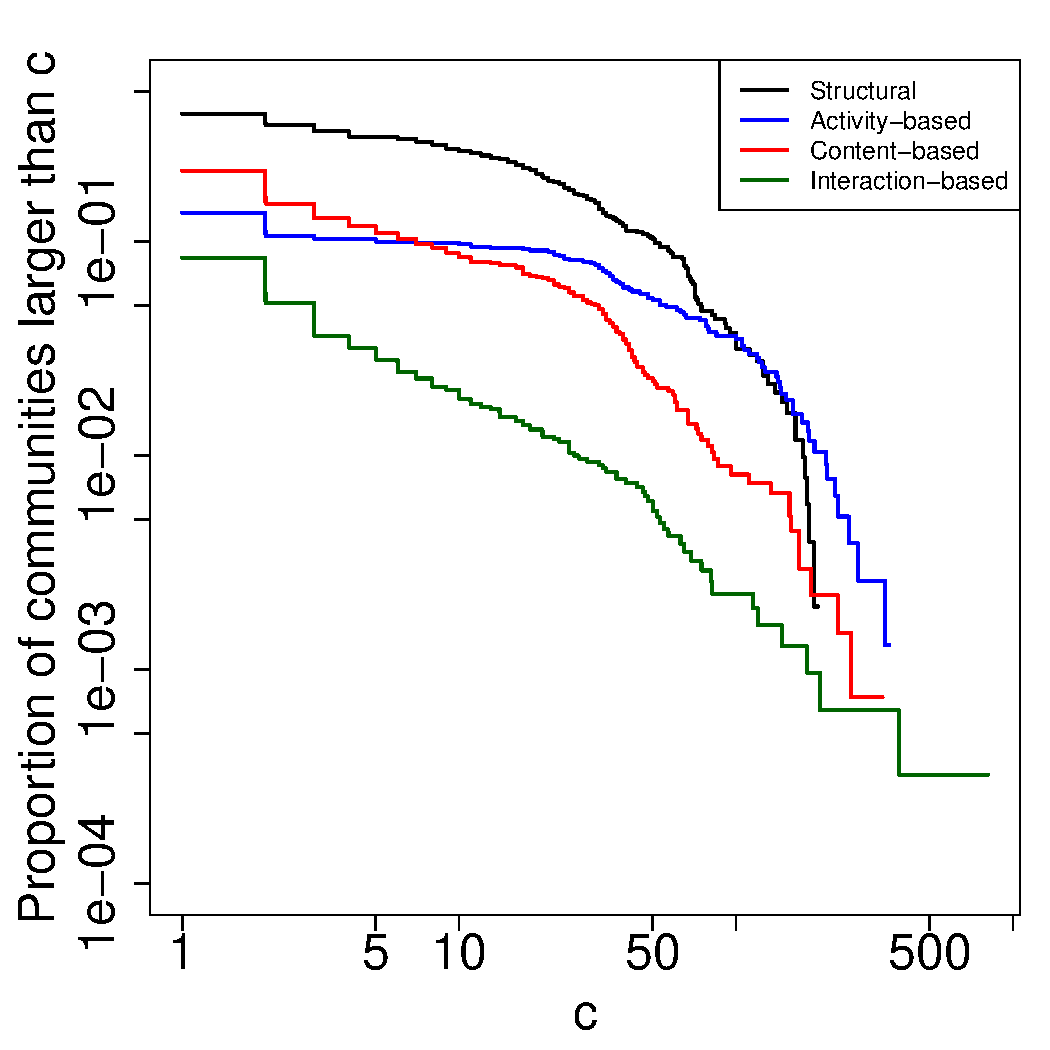
\includegraphics[width=0.50\textwidth]{Figures/comm_sizes_ecdf_loglog.pdf}
\caption{The proportion of communities greater than $c$ in size, across the different community types. Note the logarithmic scale on the horizontal and vertical axes.}
\label{Fig-community_size_distribution}
\end{figure}

% Next, we compare the number of users which belong to more than one community. Figure~\ref{Fig-overlap_plot} shows the number of users belonging to 2, 3, or 4 communities. We see that as the number of mixed membership communities increases, the number of users with that number of mixed memberships decreases. This is especially true for the activity-based community \textbf{TK: speculate on what this means? Or save for the results section?}.  In addition, \textbf{TK: mention the 5, 6, and 7 cases, not included in the figure}. This corresponded to \textbf{TK: investigate which users are the high-overlap and what communities they belong to.}

% % The user with a structural overlap of 7 communities was 1630261,
% %	https://twitter.com/marksilva

% \begin{figure}[ht]
%   \centering
% 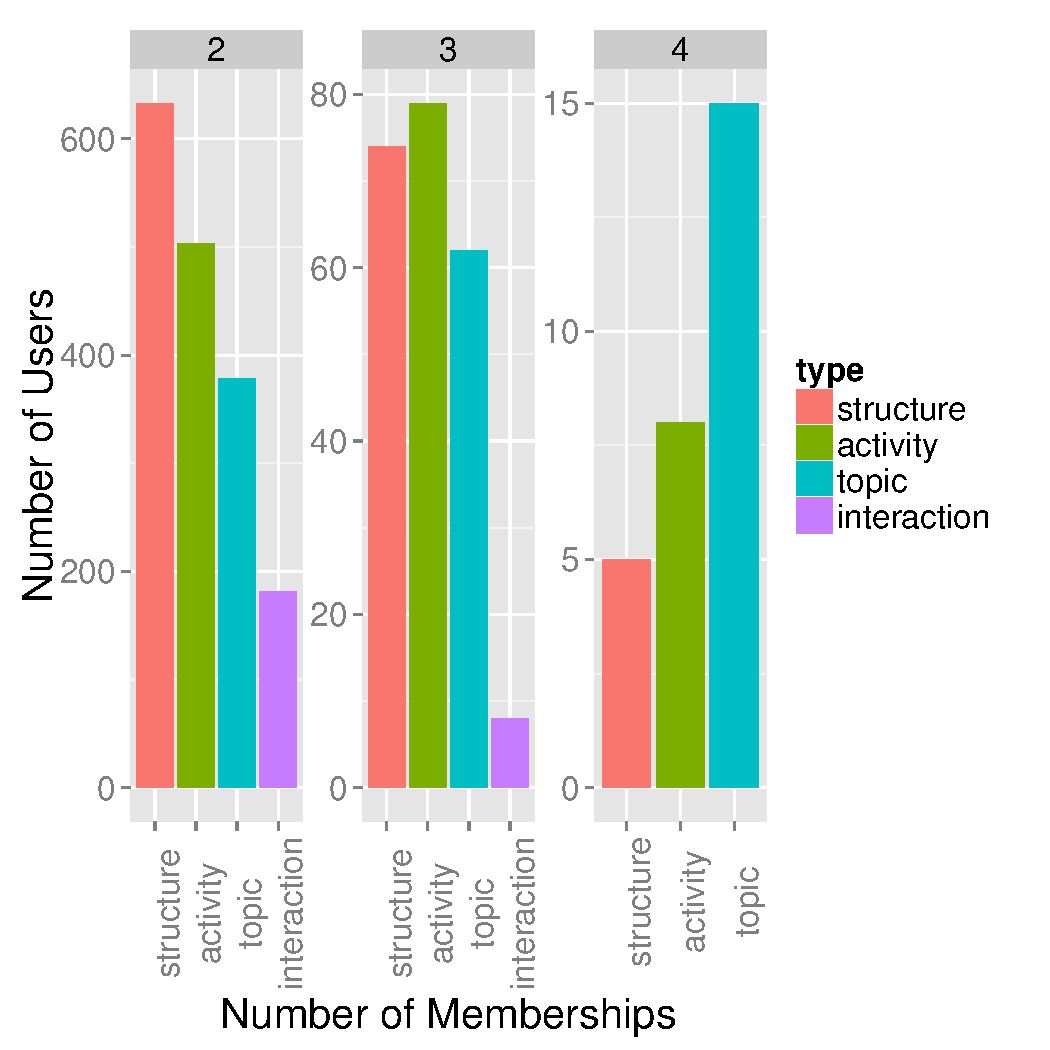
\includegraphics[width=0.50\textwidth]{Figures/overlap_by_type.pdf}
% \caption{The number of users belonging to 2, 3, or 4 communities, by community type.}
% \label{Fig-overlap_plot}
% \end{figure}

\subsection{Comparing Community Structure with Normalized Mutual Information}

In the previous section, we saw that the large scale statistics of the communities were highly dependent on the type of community under consideration. However, macroscale network statistics do not account for differences in community structure that result from operations such as splitting or merging of communities. Moreover, this view does not account for which users belong to which communities, and in particular which users belong to the same communities across community types. To answer this question, we invoke methods for cluster comparisons: given two different clusterings of nodes into communities, how similar are the two clusters? The standard approach to answering this question is to define a metric on the space of clusterings.  Because OSLOM detects \emph{coverings} rather than \emph{partitions} of users, standard cluster comparison metrics like variation of information~\cite{meilua2003comparing} are not appropriate. Instead, we use a generalization of variation of information first introduced in~\cite{lancichinetti2009detecting}, the normalized mutual information. The normalized mutual information stems from treating clustering as a community identification problem: given that we know a node's community membership(s) in the first clustering, how much information do we have about its community membership(s) in the second clustering, and vice versa? Consider the two coverings $\mathcal{C}_{1}$ and $\mathcal{C}_{2}.$We think of the community memberships of a randomly chosen node in $\mathcal{C}_{1}$ as a binary random vector $\mathbf{X} \in \{0, 1\}^{|\mathcal{C}_{1}|}$ where the $i^{\text{th}}$ entry of the vector is 1 if the node belongs to community $i$ and 0 otherwise. Similarly, $\mathbf{Y} \in \{ 0, 1\}^{|\mathcal{C}_{2}|}$ is a binary random vector indicating the community memberships of the node in $\mathcal{C}_{2}$. Then the normalized mutual information is defined as
\begin{align}
	\text{NMI}(\mathcal{C}_{1}, \mathcal{C}_{2}) = 1 - \frac{1}{2} \left( \frac{H[\mathbf{X} | \mathbf{Y}]}{H[\mathbf{X}]} + \frac{H[\mathbf{Y} | \mathbf{X}]}{H[\mathbf{Y}]}\right)
\end{align}
where $H[\cdot]$ is a marginal entropy and $H[\cdot | \cdot]$ is a conditional entropy. The normalized mutual information varies from 0 to 1, attaining the value of 1 only when $\mathcal{C}_{1}$ and $\mathcal{C}_{2}$ are identical coverings up to a permutation of their labels. See the appendix of~\cite{lancichinetti2009detecting} for more details.

We considered the normalized mutual information between the communities inferred from the structural network and the networks weighted with lag 1 through 6 transfer entropies, hashtag similarity, and mention, retweet, and mention-retweet activity. The resulting $\text{NMI}(\mathcal{C}_{i}, \mathcal{C}_{j})$ are shown in Figure~\ref{Fig-compare_coverings}. We see that similarity between the coverings is dictated by the generic community type (structural, activity-based, etc.). That is, the transfer entropy coverings are more similar to each other than to any of the other coverings, with a similar result for the mention, retweet, and mention-retweet coverings. Interestingly, the coverings resulting from the different weightings are all more similar to each other than to the structural covering from the unweighted network. Also note that the covering based on the hashtag similarities are different from all of the other weight-based coverings.

\begin{figure}[ht]
  \centering
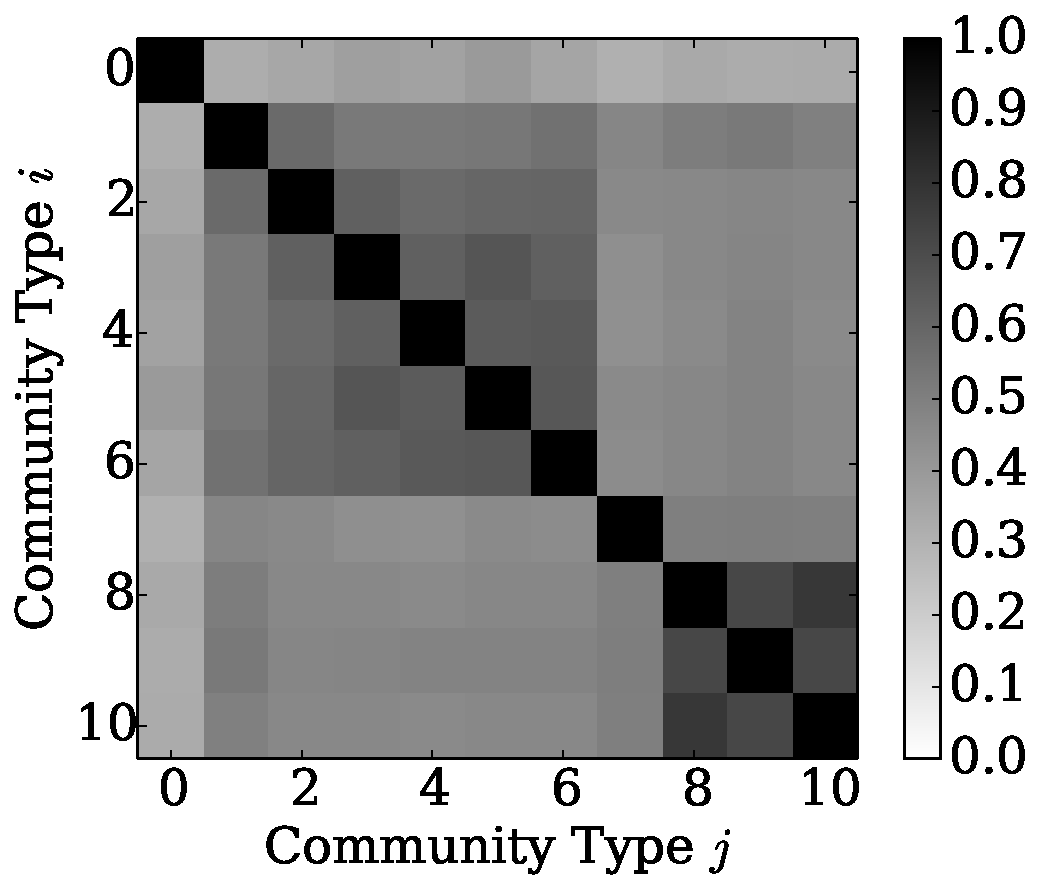
\includegraphics[width=0.50\textwidth]{figures/nmi_singletons.pdf}
\caption{The normalized mutual information between the communities using the different weightings. Weighting 0 corresponds to the structural (binary weighting) network, weightings 1 through 6 correspond to the weighting using the transfer entropies with lag 1 through 6, weighting 7 corresponds to the hashtag similarity, and weightings 8, 9, and 10 correspond to the mention, retweet, and mention-retweet weightings. Values of normalized mutual information close to 1 indicate similarity in the community structure, while values close to 0 indicate dissimilarity. The normalized mutual information is computed with the singletons removed.}
\label{Fig-compare_coverings}
\end{figure}

Thus, we see that although the activity-based, interaction-based, and topic-based communities relied on the structural network, their community structure differs \emph{the most} from the community structure of the follower network. This agrees with the results from the previous section, and reinforces that the follower network is a necessary but not sufficient part of detecting communities in online social networks.

\subsection{Comparing Edges Across Different Community-Types}

We have defined communities using four different criteria: structure, activity, interaction, and content. For a fixed community type, edges for a particular community may be partitioned into three sets: those from a node in the community to another node in the community (internal-to-internal), those from a node in the community to a node outside of the community (internal-to-external), and those from a node outside the community to a node inside the community (external-to-internal). See Figure~\ref{Fig-edge_types} for a schematic of this edge partitioning. For a meaningful community, we expect the distribution of weights within the community (internal-to-internal weights) to be different from the distribution of weights without the community (internal-to-external and external-to-internal).

\begin{figure}[ht]
  \centering
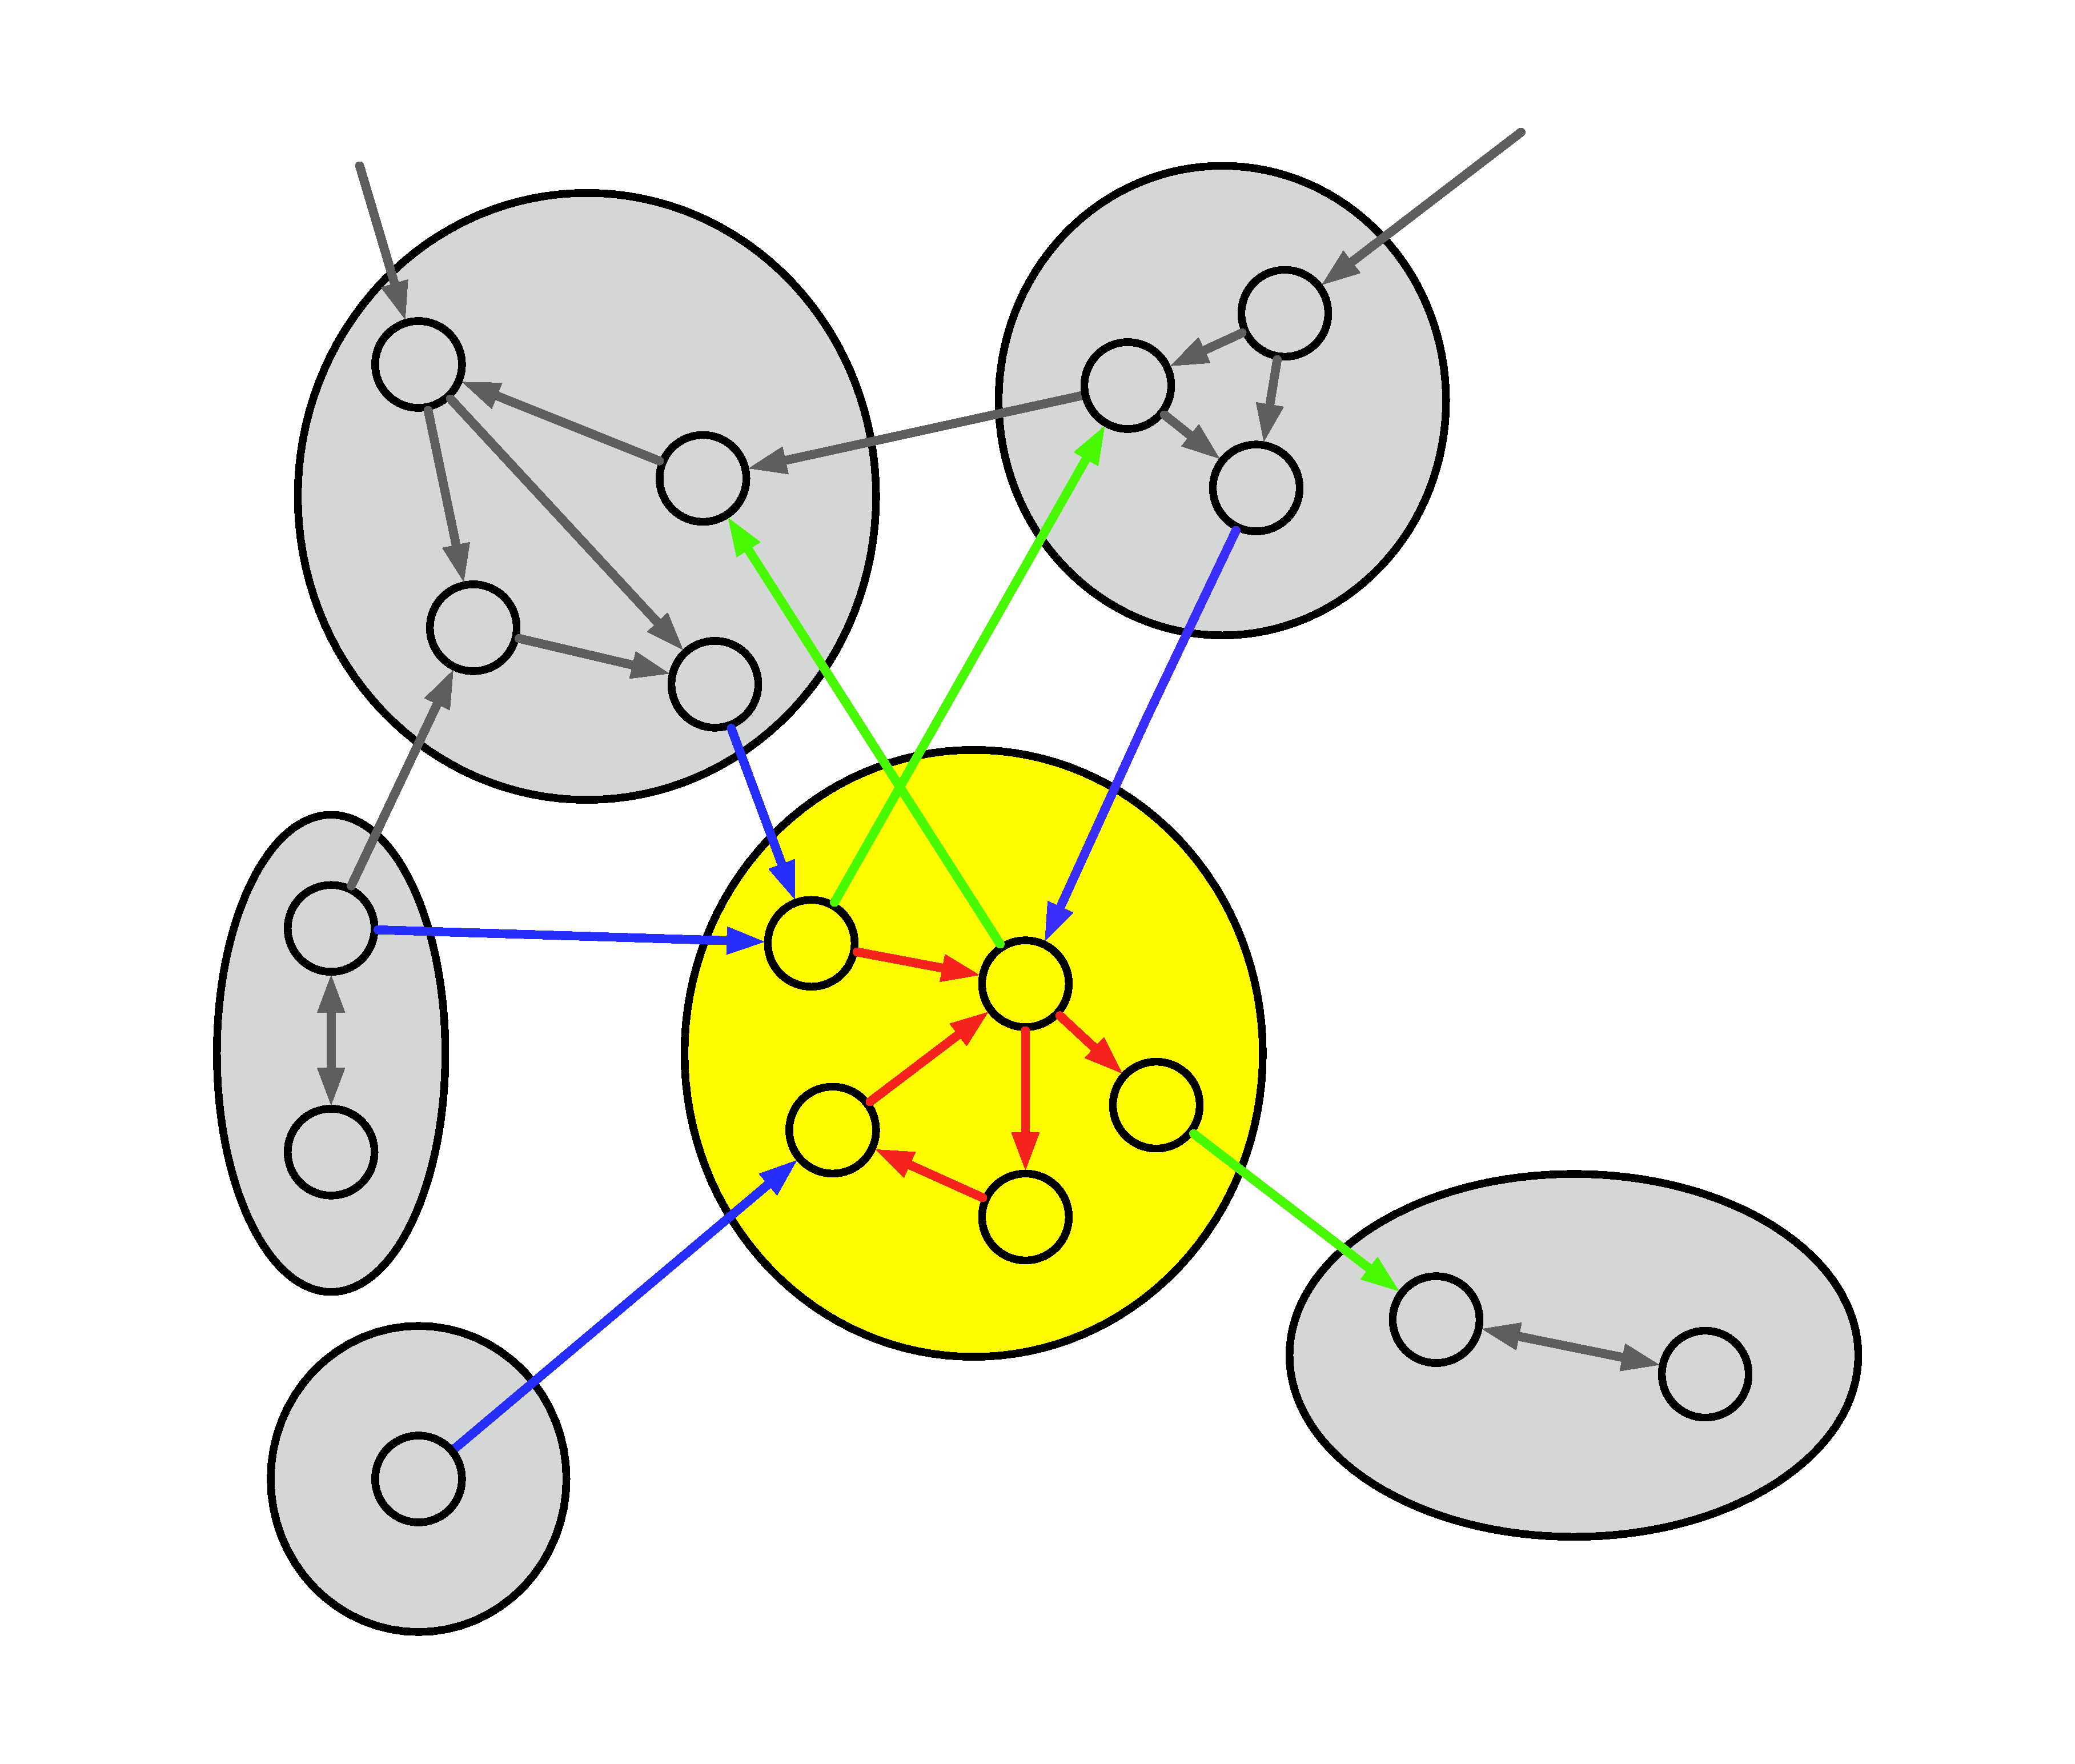
\includegraphics[width=0.50\textwidth]{figures/edge-types.eps}
\caption{An example of the edges considered in determining the edge weight distribution for a given community (the focal community is in yellow). We focus on the internal-to-internal (red), internal-to-external (green), and external-to-internal (blue) edges. For a given focal community, all other edges (grey) are not considered.}
\label{Fig-edge_types}
\end{figure}

For example, Figure~\ref{Fig-dist_across_community} shows the distributions of hashtag-based weights for the largest community defined by the mention-retweet network. We see that the distribution of internal-to-internal hashtag weights has a longer tail than either the external-to-internal or internal-to-external hashtag weights, with edges within the community having higher weights than edges crossing the boundary of the community. Thus, while the community was defined in terms of interactions, we still see a shift in the distribution of \emph{topic-similarity}.

\begin{figure}[ht]
  \centering
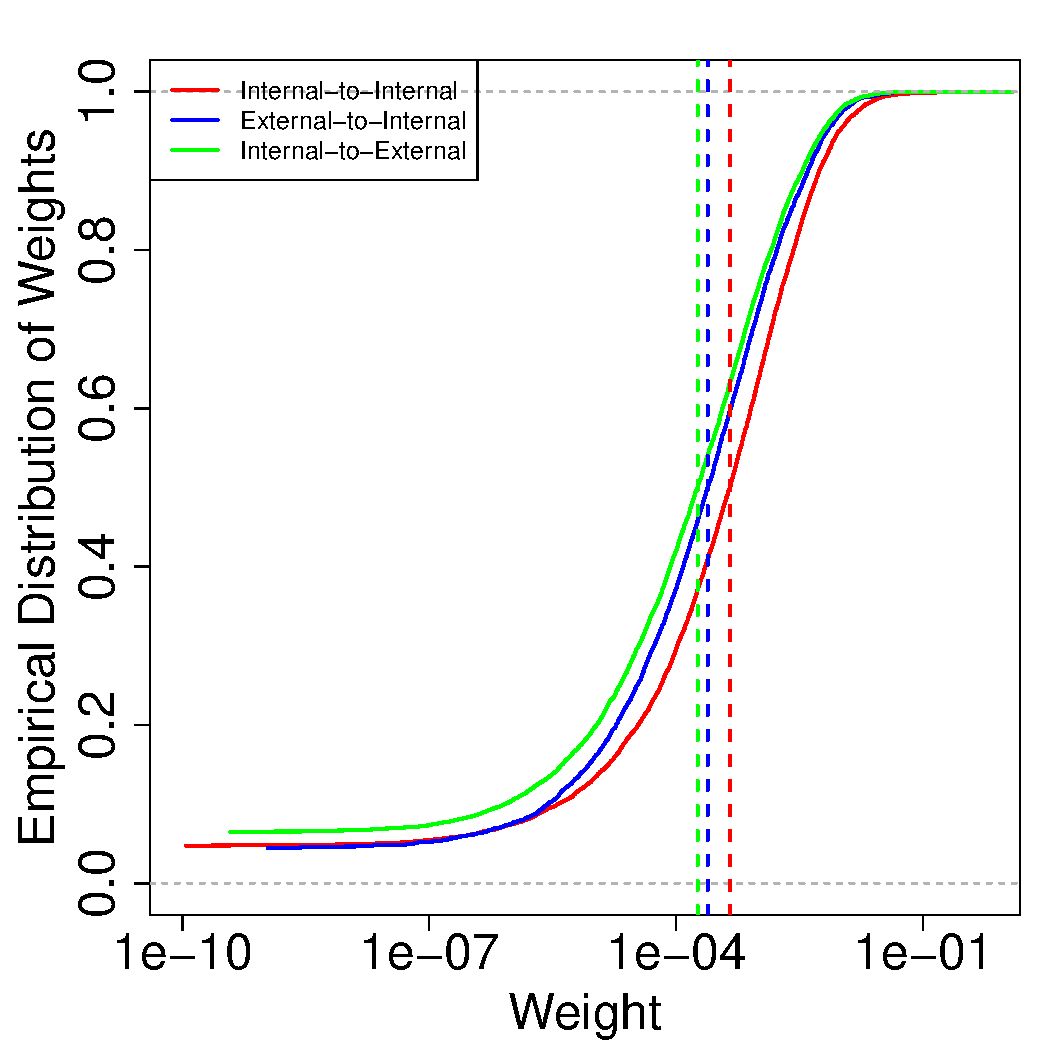
\includegraphics[width=0.50\textwidth]{Figures/comm0_labels-mention-retweet_weights-hashtag-ecdf.pdf}
\caption{The proportion of edges with a weight at least as large as the weight on the horizontal axis, across the types of edges described in Figure~\ref{Fig-edge_types}. The community is defined by user interactions, and the edge weights are determined by topics.}
\label{Fig-dist_across_community}
\end{figure}

This shift in the distribution was typical of many of the community type / weight pairings. To explore this further, for each of the top 100 largest communities defined by a particular community type (structure-based, behavior-based, content-based, or activity-based), we computed the median internal-to-internal, external-to-internal, and internal-to-external weight for that community for each weight type. These values summarize the typical value of each of these types of edges. We can then compute the ratio of the median internal-to-internal weight and the median external/internal-to-internal/external weight, which captures the proportional shift in the distribution. Finally, we compute the median of this proportional shift across all 100 of the largest communities. These values are summarized in Table~\ref{Table-medians}.

% \begin{table}
% 	\caption{The median value for the ratio of the median external/internal-to-internal/external weight to median internal-to-internal weight for the different community/weight pairings.}
% 	\centering
% 	\begin{tabular}{c | c | c  c  c  c}
% 		& & \multicolumn{4}{ c }{Community} \\ \hline
% 		\multirow{4}{*}{Weight} & & S & TE & MR & HT \\ \hline
% 		& TE & $0.0 / 0.0$ & $0.0 / 0.0$ & $0.0 / 0.0$ & $0.0 / 0.0$\\
% 		& MR & $0.0 / 0.0$ & $0.0 / 0.0$ & $0.0 / 0.0$ & $0.0 / 0.0$\\
% 		& HT & $0.0 / 0.0$ & $0.0 / 0.0$ & $0.0 / 0.0$ & $0.0 / 0.0$
% 	\end{tabular}
% \end{table}

\begin{table}
	\label{Table-medians}
	\caption{The median value across the 100 largest communities for the ratio of the median internal-to-internal weight to median external/internal-to-internal/external weight for the different community/weight pairings. \\ * For mention-retweet weights, weight zero edges were excluded from the computation of the median.}
	\centering
	\begin{tabular}{c | c | c  c  c}
		& & \multicolumn{3}{ c }{Weight} \\ \hline
		\multirow{4}{*}{Community} & & TE & MR & HT \\ \hline
		& S & $0.96/0.94$& $1.7/2.1$*& $9.0/8.0$\\
		& TE & $1.0/0.96$& $1.5/2.4$*& $24/17$\\
		& MR & $0.83/0.86$& $3.2/4.4$& $10/8.5$\\
		& HT & $0.9/0.89$& $2.4/2.6$*& $28/26$
	\end{tabular}
\end{table}

We see that overall, the 

\subsection{Qualitative Analysis}

In order to further explore the differences between the communities obtained through the various weightings, we also performed a qualitative analysis of such communities. Some interesting examples are, for instance, communities in the topic-based network such as one composed of 83 users who talk about environmental issues and frequently use hashtags such as \#green, \#eco and \#sustainability, and another one 47 users talking about small businesses and entrepreneurship, characterized by hashtags such as \#smallbiz, \#marketing and \#enterpreneur. In both cases most members of the topic-based communities are not found in the same community in the other networks, indicating that these people talk about the same things and can therefore be considered a thematic community, but do not strongly interact with each other nor behave the same, and so belong to different social groups with respect to interactions and behavior. Another interesting example is the one of a community thematically focused on Denver and Colorado, whose users do not belong to the same community in the interaction networks, but most of them do belong to the same community in the information based network. This indicates that these users react on the same events and issues regarding Colorado and are therefore strongly connected in the topic-based and in the activity-based networks, but at the same time they do not directly interact with each other and are therefore more loosely connected in the interaction-based networks, where they belong to different communities.